%\motto{Use the template \emph{chapter.tex} to style the various elements of your chapter content.}
\chapter{Physikalische Grundlagen}
\label{physics} % Always give a unique label

\chapterauthor{Amanda Hagan, Lucie Hartmann, Leon Lukacin, Ole Pross}

\abstract{some abstract}

\section{(Einführung in die Quantenmechanik für das Quantencomputing)}
\subsection{Motivation und Abgrenzung zur klassischen Physik }
\subsection{Wichtige Konzepte der Quantenmechanik }
\subsubsection{\textit{\textit{Zustände und Wellenfunktion} }}

Ein Zustand beschreibt in der Physik die Menge aller physikalisch relevanten Informationen, die ein spezifisches System charakterisieren.\\

In der klassischen Mechanik wird der Zustand eines Objektes, im einfachsten Fall eines einzelnen Teilchens, über den Ort und Impuls des Objektes beschrieben. Aus diesen Informationen lassen sich alle physisch messbaren Eigenschaften des Objektes berechnen. Dieses Modell zur Zustandsbeschreibung reicht aufgrund von Quantenmechanischen Phänomenen allerdings nicht mehr aus, um auch Quantenobjekte vollständig zu beschreiben.\\

Der Zustand eines Quantenobjektes ist über die Wellenfunktion $\Psi$ (Psi) vollständig definiert. $\Psi$ ist dabei eine komplexe Funktion, ihre Funktionswerte stammen also aus dem Zahlenraum $\mathbb{C}$. In einem durch eine Wellenfunktion $\Psi$ beschriebenen Quantensystem ist die Wahrscheinlichkeitsdichte $P(x)$ das Teilchen in Zustand $\Psi(x)$ an der Stelle $x$ zu finden $|\Psi(x)|^2$. Dies ist notwendig, damit man als Ergebnis für die Wahrscheinlichkeit eine reale nicht negative Zahl erhält. Da die Summe der Wahrscheinlichkeiten dieser Art zusammengerechnet 1 ergeben muss, muss die Wellenfunktion normalisiert sein. Dies ist der Fall, da bei einer Messung das Teilchen mit einer Wahrscheinlichkeit von 1 irgendwo gefunden wird.

\subsubsection{\textit{(Observable und Messung)??}} 
\subsubsection{\textit{Zeitentwicklung und Schrödingergleichung} }

\section{Zentrale Quantenphänomene }
\subsection{Superposition }

Welle-Teilchen-Dualismus \\

Der Welle-Teilchen-Dualismus ist ein fundamentales Konzept der Quantenmechanik, das beschreibt, dass subatomare Teilchen wie Photonen oder Elektronen gleichermaßen Wellen- und Teilcheneigenschaften besitzen. Dies widerspricht den Konzepten der klassischen Physik, in der Wellen und Teilchen getrennte Kategorien darstellen. \\

Das zentrale Experiment zum Nachweis des Welle-Teilchen-Dualismus ist das Doppelspaltexperiment. Dabei wird ein Strom Photonen durch zwei eng beieinanderliegende Spalte (Doppelspalt) auf einen dahinterliegenden Schirm gelenkt. Dabei entsteht auf dem Schirm ein Interferenzmuster. Dies ist ein Effekt typisch für  Wellen, die Interferenz ist dabei die Summe der Amplituden einzelner Wellen. Der Welleneffekt mit dem Interferenzmuster bleibt sogar bestehen wenn die Teilchen einzeln abgeschossen werden. Daraus kann gefolgert werden, dass Teilchen sich wie Wellen verhalten, welche durch die beiden Spalten miteinander inferieren. Das Interferenzmuster verschwindet allerdings bei dem Versuch den Weg eines Teilchens durch Messung zu bestimmen. In diesem Fall der Messung verhält sich das Teilchen klassisch, wie man es von einem Teilchen erwarten würde und der Welleneffekt geht verloren. Somit konnte neben dem Verhalten als Teilchen und Welle nachgewiesen werden, dass der Akt der Messung den Zustand des eines Objektes in einem quantenmechanischen System beeinflusst. \\

Heisenbergsche Unschärferelation \\

Die Heisenbergsche Unschärferelation ist ein weiteres zentrales Prinzip der Quantenmechanik und wurde 1927 von Werner Heisenberg formuliert. Sie beschreibt eine fundamentale Grenze der gleichzeitigen Bestimmbarkeit bestimmter Paare von physikalischen Größen, beispielsweise des Ortes- und des Impulses eines Teilchens. Die Unschärferelation sagt nicht aus, dass Messgeräte zu ungenau sind um diese Werte zu bestimmen, sondern dass die Unschärfe eine fundamentale Eigenschaft der Quantenmechanik ist. Sie resultiert aus der Wellencharakteristik von Teilchen in der Quantenmechanik. Je genauer der Ort durch eine bestimmte Wellenfunktion ermittelt wird, desto größer ist die Breite an Werten für den Impuls des Teilchens. Die Unschärferelation stellt damit eine Abkehr vom Determinismus der klassischen Physik dar, in dem alle physikalischen Größen beliebig genau bestimmt werden können. Stattdessen legt die Unschärferelation die Grundlage für die probabilistische Natur quantenmechanischer Systeme und Zustände. \\

Superposition\\

Die Superposition in der Quantenmechanik ist ein Phänomen, welches unter anderem aus diesen quantenmechanischen Effekten resultiert. Die Superposition besagt, dass sich ein Quantensystem gleichzeitig in mehreren möglichen Zuständen befindet. Dies hält an, bis eine Messung durchgeführt wird. Mathematisch wird dies durch die Überlagerung mehrerer Wellenfunktionen beschrieben, also der Linearkombination der Wellenfunktionen der einzelnen Zustände. Die Zustände haben dabei jeweils einen eigenen Wahrscheinlichkeitsanteil.
Bei der Messung erfolgt der Kollaps dieser Wellenfunktion in einen eindeutigen Zustand. Beim Kollaps der Wellenfunktion ist der gemessene Zustand von dieser Wahrscheinlichkeit abhängig Ein Teilchen, zum Beispiel ein Elektron, kann sich somit in einer Überlagerung verschiedener Orte und Impulse befinden. Nach der Heisenbergschen Unschärferelation ist es dabei prinzipiell nicht möglich, beide Eigenschaften gleichzeitig exakt zu bestimmen.\\

Es gibt mehrere Beispiele, um das Prinzip der Superposition zu verdeutlichen. Das bekannteste Gedankenexperiment zur Veranschaulichung der Superposition ist Schrödingers Katze: Eine Katze wird zusammen mit einer Ampulle voll Gift  in eine nicht einsehbare Box gesperrt. Die Ampulle wird durch den zufälligen Zerfall eines radioaktiven Teilchens zerstört. Die Katze befindet sich, solange keine Beobachtung erfolgt, aus Sicht des Betrachters in einer Superposition aus lebendig und tot. Also in einer Überlagerung mehrerer Zustände gleichzeitig. Ein einfacheres Beispiel ist ein Münzwurf. Bei einem Münzwurf ist die Münze während sie in der Luft ist in einer Superposition aus den Zuständen Kopf und Zahl. Erst bei der Messung wird ein eindeutiger Zustand ermittelt.\\

\begin{itemize}
\item Licht verhält sich wie Welle (Doppelspaltexperiment) und Teilchen (Photon)
\item Welle Teilchen Dualismus
\item Beispiel mit Schrödingers Katze
\item In beiden Zuständen bis gemessen wird
\item Teilchen z.B. an zwei Orten gleichzeitig, aber auch andere (sich ausschließende) Eigenschaften parallel -> Superposition -> Teilchen in allen möglichen Zuständen gleichzeitig
\item Einwirkung von außen oder Messung zerstört Superposition
\item Heisenbergsche Unschärferelation
\item Beide Zustände der Superposition haben jeweils einen Anteil, der genaue Wert eines Anteils ist nicht bekannt
\item Mit einer Wahrscheinlichkeit abhängig vom Anteil nimmt ein Teilchen einen der beiden Zustände an

\item Schrödingergleichung/Wellenfunktion
\item Linearkombination (widersprüchlicher) Zustände z.B. 0 und 1/ tot und lebendig
Bei Messung erfolgt Kollaps der Wellenfunktion -> am Ende ein Zustand
\item Wellenfunktion beschreibt ein quantenmechanisches System und enthält alle Informationen über dieses System
\item Eigenvalues und Eigenstates
\end{itemize}

\subsection{Quanteninterferenz}

\begin{itemize}
\item Interferenzmuster aus Doppelspaltexperiment -> Wahrscheinlichkeitsamplitude
Wahrscheinlichkeitsamplituden können sich verstärken oder auslöschen (konstruktiv/destruktiv)
\item Interferometer
\item Einzelnes Photon löst allein Interferenz aus -> entgegen Intuition -> Photon muss in Superposition sein
\item Messung zerstört Verhalten als Welle -> nur noch als Teilchen
Nutzbar in Gattern
\item Tunneleffekt
\end{itemize}

\subsection{Verschränkung }

Das Konzept der Verschränkung (engl. ``entanglement'') beschreibt gewissermaßen die Korrelation mehrerer Qubits miteinander, das heißt sie hängen in einem besonderen Maße zusammen. \\
Für einen erleichterten Einstieg soll ein Beispiel anhand zweier gewöhnlicher Münzen gemacht werden. Werden zwei gewöhnliche Münzen geworfen, hat man vier mögliche Ausgänge für den Münzwurf, bei denen H für Kopf und T für Zahl stehen sollen: HH, HT, TH, TT. \\
Alle Varianten der Ausgänge haben hierbei eine identische Wahrscheinlichkeit von 25\%. Sind diese zwei Münzen jedoch in einem verschränkten Zustand  $\frac{1}{\sqrt{2}} \left( \lvert HH \rangle + \lvert TT \rangle \right)$, sind hierbei nur zwei Ausgänge möglich, die beide jeweils eine 50\%-Wahrscheinlichkeit haben, nämlich HH oder TT. \\
Diese Verschränkung ist unabhängig von der räumlichen Nähe der Münzen und kann über große Distanzen hinweg wirken. Weiß man das Ergebnis der einen Münze, so weiß man automatisch auch immer das Ergebnis der anderen Münze. Im Bereich der Quantenmechanik ist genau dies bezogen auf diverse Teilchen anstelle der Münzen möglich. 
Das Phänomen der Verschränkung ist jedoch ein reines Quantenphänomen, das keine Erklärung in der klassischen Physik besitzt. \\
Eine Vermutung über die Natur der Verschränkung besteht aus der sofortigen Informationsübertragung zweier Teilchen, die über die Schnelligkeit der Lichtgeschwindigkeit hinausgeht, was jedoch als widerlegt gilt. Stattdessen teilen Teilchen nicht-klassische Information während der Verschränkung, die im Messprozess beobachtet werden kann. \\
Eine weitere frühe Interpretation, bekannt unter dem Namen ``Hidden Variable Theory'', nahm an, dass Teilchen beim Erzeugen mit verbogenen Eigenschaften erschaffen werden, die Messergebnisse deterministisch bestimmen. Beispielsweise wäre hierfür der Zerfall eines Teilchens in zwei Teilchen. Auf Basis der Impulserhaltung kann man durch die Messung des Impuls des einen Teilchens auf den Impuls des anderen Teilchens schließen, da der Gesamtimpuls vorher bekannt ist. 
\cite{hughes_quantum_2021}
% Quantum Computing for the Quantum Curious - Hughes et al. - 2021
\\

Das Problem dieser Theorie findet sich jedoch in Bell's Theorem, das zeigt, dass wenn die Welt durch diese versteckten Variablen beschrieben wäre, gewisse mathematische Ungleichungen in Experimenten eingehalten werden müssten. 
Diese gelten als Einschränkungen für alle lokal-realistischen Theorien, d.h. Theorien, die annehmen, dass Lokalität und Realismus gelten. \\
Lokalität bedeutet hierbei, dass es keinen Einfluss gibt, der sich schneller als mit Lichtgeschwindigkeit ausbreiten kann. \\
Realismus bezieht sich auf die Annahme, dass physikalische Größen zu jedem Zeitpunkt definierte Werte besitzen, unabhängig davon, ob diese gemessen werden. 
Die quantenmechanische Verschränkung erfüllt diese Annahmen durch die ``spukhafte Fernwirkung'' jedoch nicht, da es eine scheinbar unmittelbare Verbindung über sehr große Distanz hinweg gibt. Dem Lokalitätsprinzip entsprechend, könnten zwei Systeme sich nur dann beeinflussen, wenn sie einen Kontakt oder ein physikalisches Feld haben, das sie verbindet. Quantenobjekte haben jedoch durch die mangelnde Lokalität keine klassische Kausalität, sondern nur die Beobachtung, dass die Ergebnisse immer korrelieren, auch wenn sie räumlich weit voneinander getrennt sind.

Da die Grenzen der Bell-Ungleichung also nicht auf gemessene Experimente zutreffen, kann keine lokal-realistische Theorie das quantenmechanische Phänomen der Verschränkung erklären. Die Resultate stimmen mit der Quantenmechanik überein, anstatt mit lokalen Theorien wie der Hidden Variable Theory. 

Basierend hierauf ergibt sich das Dilemma, dass Realismus und Lokalität nicht beide gleichzeitig gelten können. Diese Schlussfolgerung führt jedoch zu tiefergehenden philosophischen Fragen über die Realität, die an dieser Stelle nicht weiter behandelt werden sollen.
Unabhängig davon findet die Verschränkungen Anwendungen in moderner Quantentechnologie, wie in der Quantenkryptographie oder Quanten-Teleportation.  
\cite{homeister_quantum_2022}
% Quantum Computing verstehen: Grundlagen - Anwendungen - Perspektiven - Homeister - 2022
\\

Um ein Beispiel für die Quantenverschränkung in der Praxis zu machen, soll an dieser Stelle noch  die spontane parametrische Fluoreszenz (engl. ``spontaneous parametric down-conversion, SPDC'') genannt werden. Bei diesem Prozess trifft ein Photon aus einem Laser auf ein nichtlineares Kristallmaterial. Dadurch spaltet sich das Photon in zwei neue Photonen, wobei die Polarisation der neuen Photonen miteinander verschränkt sind, sodass man typischerweise folgenden Zustand erhält:
$\frac{1}{\sqrt{2}} \left( \lvert H \rangle_A \lvert H \rangle_B + \lvert V \rangle_A \lvert V \rangle_B \right)$
Misst man also die Polarisation des Photons A, kennt man ebenfalls die Polarisation des Photons B, jedoch ohne dass dies klassisch bereits festgelegt war.
\cite{hughes_quantum_2021}
% Quantum Computing for the Quantum Curious - Hughes et al. - 2021



\section{Quantenmessung }
\subsection{Grundlagen der Quantenmessung (projektive Messungen, Messoperatoren)}

Die Messung in der Quantenmechanik unterscheidet sich grundlegend von der Messung in der klassischen Physik, einerseits durch die Auffassung der Grundkonzepte der Quantenmechanik, andererseits durch die mathematische Beschreibung und Interpretation der Messergebnisse.
In der klassischen Welt wird das Verhalten eines Systems nicht durch das alleinige Beobachten des Systems beeinflusst; ein Ball beispielsweise wird sein Verhalten und seine Flugkurve nach einem Schuss nicht verändern, unabhängig davon, ob jemand dabei zusieht oder nicht.
In der Quantenwelt hingegen sind die gemessenen Objekte (z.B. Photonen) winzig klein und die entsprechenden Messgeräte verhältnismäßig groß, sodass schon alleine deshalb die Messung zwangsläufig den Zustand eines Quantensystems beeinflussen wird. 
Dass eine Messung den Zustand des Quantensystems verändert und das Ergebnis dieser Messung zufällig ist, ist im Rahmen des zweiten Postulats der Quantenmechanik eine zentrale Annahme, die in diesem Kapitel weiter erörtert werden soll. Als Observablen- oder Messwertpostulat ist es das zentrale Postulat für die Messung im gegebenen Rahmen.

Das zweite Postulat besagt, dass eine Quantenmessung einer Projektion des Zustandes $\ket{\psi}$ auf eine Basis $\ket{|v_i|}$ entspricht. Mit der Wahrscheinlichkeit $|\braket{v_i|\psi}|^2$ erhalten wir das Ergebnis $v_i$. Das System befindet sich dann im Zustand $\ket{v_i}$. \cite{lvovsky_quantum_2018} 
% Lvovsky - Quantum Physics - 2018 - Kapitel 1.4.1 The Measurement Postulate
\newline Dieses Konzept wird auch 'projektive Messung' genannt, da die Messung des Zustandes auf einen Basiszustand projiziert wird, wobei die Begriffe der Projektion und der Basiszustände noch weiter erläutert werden sollen. \\
\\

Ein Quantensystem wird innerhalb einer bestimmten Basis gemessen.Der Begriff 'Basiszustand' bezieht sich hierbei auf die möglichen Zustände eines Systems, die insgesamt die Basis bilden (beispielsweise $\ket{v_1}$ oder $\ket{v_2}$) und bei der Messungen angenommen werden können.
Beim Messen springt das System in einen der Basiszustände. 
Wird hierbei der Wert $v_i$ gemessen, so springt das System in den Zustand $\ket{v_i}$. Das Messergebnis ist also der Zustand $\ket{v_i}$. 
Dabei wird die Information, welche Zustände gemessen werden und welche entsprechenden Zahlenwerte ihnen zugeordnet werden, in einem 'Observable Operator' zusammengefasst. 
Dieser Observable Operator, der die Basis der Messungen beschreibt und die möglichen Werte der Messung enthält, kann folgendermaßen dargestellt werden: \\
\\
\begin{equation}
\hat{V} = \sum_i v_i \, \ket{v_i}\bra{v_i}
\end{equation}.
\\ 
\\
Jeder Zustand $\ket{v_i}$ ist hierbei ein Eigenzustand dieses Operators. Der dazugehörige Eigenwert $v_i$ ist der Zahlenwert der Messung, den man bei der Messung des Zustandes erhält. 
Die Zuordnung eines Wertes ist für einige Messgrößen (bspw. der Ort eines Teilchens im Raum) natürlich, für andere (z.B. die Polarisation eines Photons) weniger. Trotzdem wird auch in weniger natürlichen Fällen  eine Zahl zugeordnet, so beispielsweise
+1 für eine horizontale $\ket{H}$ und -1 für eine vertikale $\ket{V}$ Polarisation. Eine Observable kann für jede messbare Größe (Ort, Energie, Puls, Spin, etc.) definiert werden. Eine Ausnahme bildet hierbei die Zeit, da diese in der Quantenmechanik nicht als Observable definiert und behandelt wird.
Daher gibt es keinen Zeit-Operator oder Eigenzustände der Zeit. Die Zeit dient lediglich als kontinuierliche Variable zur Beschreibung der Entwicklung des Quantensystems. 
\cite{lvosvsky_quantum_2018} 
% Lvovsky - Quantum Physics - 2018 - Kapitel 1.9.1 Observable Operators
\\
\\

Projektive Messungen werden also durch eine Observable M beschrieben. Seien die Eigenwerte m die möglichen Ergebnisse der Messung und $P_m$ die zugehörigen Projektoren, kann M geschrieben werden als:
\begin{equation}
    M = \sum_m mP_m
\end{equation}
Hierbei sind $P_m$ die orthogonalen Projektoren auf den Eigenraum von M. Jeder Projektor projiziert auf einen Unterraum des Hilbertraums, der zu einem bestimmten Eigenwert m gehört. Diese Formel bildet die verallgemeinerte Darstellung der zuvor genannten Formel zur Darstellung der Observablen. % Check & umschreiben
Es gelten daraus folgende Grundregeln: \\ \\
\begin{enumerate}
\item Die Gesamtwahrscheinlichkeit aller Messungen (Projektoren) ergeben in Summe 1, d.h. sie decken den gesamten Zustandsraum ab. Jeder mögliche Zustand wird durch eine Kombination der Projektoren beschrieben und bildet in Summe den Einheitsoperator. \\
\item Die Wahrscheinlichkeit einer Messung m ergibt sich aus folgender Formel:
\begin{equation}
    p(m) = \langle \psi \mid P_m \mid \psi \rangle
\end{equation}
Hierbei ist p(m) die Wahrscheinlichkeit, dass die Messung des Systems im Zustand $\ket\psi$ das Ergebnis m ergibt. Das ist mathematisch das s.g. Bornsche Wahrscheinlichkeitsgesetz.
Es ist das Quadrat der Länge der Projektion von $\ket\psi$ auf den m-Unterraum. Es berechnet also die Länge der Projektion von $\ket\psi$ auf den Eigenraum von m. \\
\item Nach einer Messung mit Ergebnis m kollabiert der Zustand $\ket\psi$ in einen Zustand, der der Messung entspricht. Dies wird auch Projektionspostulat genannt. Die Projektion dieses Zustandes muss wieder normalisiert werden, um wieder einen Zustand mit der Norm 1 zu erhalten.
Da wiederholte Messungen jedoch im Bereich des Quantumcomputing geringe Relevanz hat, wird auf die wiederholte Messung nicht weiter eingegangen. \\ 
\end{enumerate}

In kurz greift man bei der Messung eines Zustandes $\ket\psi$ also nur den Teil aus dem gesamten Zustandsvektor heraus, den man misst. Es wird der Anteil extrahiert, der zugehörig zum gemessenen Eigenwert ist, also die Projektion $P_m \ket\psi$. Der Zustand wird bei der Messung also in seine Bestandteile entsprechend der verschiedenen Eigenräume zerlegt. Um hieraus wieder einen gültigen und normierten Zustand zu erhalten, muss dieser Vektor mit seiner eigenen Länge normiert werden. Da dies jedoch nur zur weiteren Arbeit mit demselben Quantensystem relevant ist, wird die Normierung nicht weiter berücksichtigt und es wird stattdessen auf wiederholte Messungen verwiesen.
\cite{kasirajan_fundamentals_2021} 
%Fundamentals of Quantum Computing: Theory and Practice – Kasirajan (Kapitel zu Projective Measurements)

Um ein Beispiel für den Messprozess und den Zerfall auf den Eigenzustand bei der projektiven Messung zu machen, soll ein Photon auf einen Polarizing Beam Splitter (PBS) treffen. Dieser lässt horizontal polarisiertes Licht passieren, aber reflektiert vertikal polarisiertes Licht.
Betrachtet man einen Lichtstrahl aus der klassischen Physik, würde man erwarten, dass dieser sich teilt - ein Teil des Lichtes würde reflektiert werden, ein anderer Teil würde passieren. Ein Photon als kleinster Teil des Lichts kann jedoch nicht weiter geteilt werden.
Dementsprechend ist das Ergebnis zufällig: das Photon wird mit einer gewissen Wahrscheinlichkeit passieren oder reflektiert werden. Das Photon entscheidet sich bei der Messung, ob es horizontal oder vertikal polarisiert sein wird und springt bei der Messung in den gewählten Zustand.
Man könnte auch sagen durch die Messung wird der Superpositionszustand auf einen der möglichen Eigenzustände reduziert. Die Superposition selbst liegt nicht im Eigenraum, sondern ist eine Überlagerung der Zustände aus den Eigenräumen, wobei ``horizontal'' und ``vertikal'' im Eigenraum mit ihrem jeweiligen Eigenwert liegen. Hierbei zerfällt der Ursprungszustand, sodass dies bei folgenden PBS nicht erneut vonstatten gehen könnte - das Photon wird den hierbei gewählten Zustand beibehalten.
Es gibt ab diesem Punkt keine weiteren zufälligen Zustandsänderungen. 
\cite{lvovsky_quantum_2018}
% Quantum Physics – Lvovsky – 2018 (Kapitel 1.4.1 The Measurement Postulate)

\subsection{Nichtdeterminismus}

Das oben beschrieben Phänomen der zufälligen Messung ist auf den Nichtdeterminismus der Quantenmessung zurückzuführen. Das bedeutet, dass das Ergebnis der Messung zufällig ist. Man erhält den Wert $\ket v_i$ mit einer gewissen Wahrscheinlichkeit.
Je besser der Zustand $\ket \psi$ zu einem Messzustand $\ket v_i$ passt, desto wahrscheinlicher ist das Ergebnis $v_i$. Mit Hilfe des Observable Operators können Werte der klassischen Statistik berechnet werden, so der Erwartungswert, die Varianz bzw. die Unschärfe der Messung (Standardabweichung). 
Klassisch statistische Kennzahlen lassen sich mit klassischen Operationen berechnen. Entsprechend ist die statistische Verteilung der Messergebnisse leicht zu berechnen. 
\\ \\
Um hierbei auf das Beispiel der Photonen zurückzukommen, führen wir ein, dass die horizontale Polarisierung des Photons dem Wert +1 zugeordnet wird, die vertikale Polarisierung dem Wert -1.
Ein diagonal polarisiertes Photon (45°) hat entsprechend eine 50\% Chance den PBS zu passieren (+1) oder reflektiert zu werden (-1). Bei der wiederholten Messung dieses Prozesses, ist der Mittelwert 0, da sich beide Superpositionen ausgleichen.
Die Varianz entspricht einem Wert von 1, da die Messung immer um +1 oder -1 vom Mittelwert (0) abweicht.
In der klassischen Physik sind solche Messungen deterministisch vorhersehbar. Für einzelne Photonen gibt es den Zufall, für eine Vielzahl von Photonen als Licht gibt es jedoch feste Erwartungen und Regeln.
Entsprechend ist es auch im Quantensystem. Mit einer Vielzahl an Photonen wird die relative Unsicherheit sehr klein und das Verhalten erscheint klassisch und stabil, obwohl die Photonen im Kleinen in Form der Einzelphotonen vom Zufall beherrscht sind.
Die Quantenfluktuationen verschwindend relativ gesehen also im großen Maßstab durch die wiederholte Messung und eine klare Wahrscheinlichkeitsverteilung.
\cite{kasirajan_fundamentals_2021}
% Quantum Physics – Lyvovsky – 2018 (Kapitel 1.9.2 Observable Operators)
\\ \\
Erwähnenswert im Rahmen der Messung ist weiterhin das 'Heisenberg Uncertainty Principle'. In der klassischen Physik ist eine Unsicherheit im Rahmen der Messung Folge eines ungenauen Messapparates, die durch eine Verbesserung des Apparates selbst verringert werden kann.
Dies gilt jedoch im Kontext der Quantenmechanik nicht. Hierbei kann ein Apparat präzise auf die Messung eines Observablen abgestimmt sein, jedoch bei der Messung einer anderen Observablen durchweg schlecht abschneiden. \\
Möchte man zwei Größen gleichzeitig messen, beispielsweise Ort und Energie oder auch verschiedene Spins, so kann das möglich sein. Hierzu müssen jedoch zwei Observablen kommutieren, d.h. mathematisch verträglich sein, um gleichzeitig messbar sein zu können. \\
Ist dies der Fall, gibt es eine bestimmte Basis von Zuständen (Eigenbasis), in der beide Observablen gleichzeitig genau bestimmt werden können. Das System in diesem Zustand verändert seinen Zustand nicht, wenn beide Größen nacheinander gemessen werden, d.h. die Observablen sind kompatibel. \\
Wenn die Observablen jedoch nicht kommutieren, so gibt es keinen Zustand, bei dem man beide Größen gleichzeitig exakt wissen kann. Misst man hierbei A, wird das Ergebnis von B zufällig sein, da die Messung von B durch die Information über A gestört ist.
Das heißt bestimmte Paare von Größen können nicht gleichzeitig beliebig genau gemessen werden. 
Zwei Größen, die nicht kommutieren, sind z.B. Ort und Impuls eines Teilchens. Je genauer man den Ort kennt, desto ungenauer lässt sich der Impuls messen und umgekehrt. 
\cite{kasirajan_fundamentals_2021}
% Quantum Physics – Lyvovsky – 2018 (Kapitel 1.9.3 Uncertainty Principle)

\subsection{Messprozess}

Ein Prozess, der im Rahmen der Messung bereits mehrfach erwähnt, jedoch bisweilen noch nicht konkret benannt wurde, ist der Kollaps der Wellenfunktion. Dieser Prozess ist zentral für die Messung. 
Unter dem Kollaps der Wellenfunktion versteht man den Vorgang, bei dem der Zustand eines Quantensystems auf einen Basiszustand 'springt', das heißt der Zustand des Systems kollabiert auf einen der möglichen Messzustände. Die Wahrscheinlichkeit für den Wert, den man beim Kollaps erhält, ist durch die bereits genannte Bornsche Regel beschrieben.
Dies zeigt die Annahme der Quantenmechanik des Nichtdeterminismus, dass der Zufall grundlegend ist. Selbst mit perfekten Geräten kann der Zustand entsprechend nicht exakt vorhergesagt werden. 
\cite{lvovsky_quantum_2018}
% Quantum Physics – Lyvovsky – 2018 (Kapitel 1.4.1 The Measurement Postulate)
\\

Ein Quantenzustand ist also nur in abgeschottetem Zustand stabil. Um aus Perspektive der Außenwelt etwas über den Zustand des Systems zu erfahren, ist jedoch eine Messung nötig, wobei der genaue Zustand nicht ermittelt werden kann.
Die Superposition selbst wird durch die Messung zerstört und ein klassischer Zustand wird angenommen und beobachtet. Diese Messung ist außerdem für verschiedene Basen möglich und es kann entsprechend nur der Zustand bzgl. einer Basis gemessen werden, sofern die folgende Messung durch den Zerfall des Systems nicht weiter möglich ist.
Da die Messung nicht rückgängig gemacht werden kann, kann durch den Kollaps der Wellenfunktion dieselbe Messung nicht wiederholt werden.
\cite{homeister_quantum_2022}
% Quantum Computing verstehen: Grundlagen – Anwendungen – Perspektiven – Homeister – 2022 (Kapitel 2.8 Das Messen von Quantenregistern)
\\

Aus diesem Phänomen ergibt sich auch das No-Cloning-Theorem. Da das System selbst bei der Messung zerstört wird, kann das Qubit nicht erneut gemessen werden. Die Superposition selbst ist für dasselbe Qubit nicht mehr vorhanden. Die Messung kann entsprechend nur für ein identisches Qubit wiederholt werden.
Folglich dieser Logik kann ein Qubit in einem unbekannten Zustand nicht kopiert werden. Dies hat wichtige Konsequenzen für die praktische Anwendung, da simple Kopien, wie sie auf klassischen Computern möglich sind, durch die zuvor notwendige Messung der bestehenden Zustände nicht ohne Weiteres auf quantenbasierten Systemen ermöglicht werden.
\cite{hughes_quantum_2021}
% Quantum Computing for the Quantum Curious – Hughes et al. – 2021 – s. 36


\section{Mathematische Beschreibung von Qubits}
\label{sec:hilbertraum}

Die präzise mathematische Erfassung von Qubits ist eine notwendige Voraussetzung für das Verständnis quantenmechanischer Informationsverarbeitung. Im Zentrum steht dabei der \textit{Hilbertraum} als fundamentale Struktur zur Darstellung physikalischer Zustände. Dieses Kapitel stellt die Konzepte vor, auf denen spätere Abschnitte über Quantengatter, Messprozesse und Algorithmen aufbauen. 

\subsection{Hilbertraum und Zustandsvektoren}

Ein Qubit wird mathematisch durch einen normierten Vektor in einem komplexen, zweidimensionalen Vektorraum beschrieben. Dieser Raum ist ein Spezialfall eines sogenannten \emph{Hilbertraums}~\cite{nielsen2002quantum, greinerQM}. Ein Hilbertraum $\mathcal{H}$ ist ein vollständiger, komplexer Vektorraum, der mit einem inneren Produkt $\langle \cdot | \cdot \rangle$ ausgestattet ist. Die Vollständigkeit garantiert, dass jede Cauchy-Folge in $\mathcal{H}$ konvergiert. Das ist eine Eigenschaft, die für die konsistente mathematische Beschreibung kontinuierlicher physikalischer Prozesse unabdingbar ist.

Das Skalarprodukt erfüllt drei zentrale Eigenschaften:
\begin{itemize}
    \item \textbf{Linearität im zweiten Argument:} $\langle \psi | a \phi_1 + b \phi_2 \rangle = a \langle \psi | \phi_1 \rangle + b \langle \psi | \phi_2 \rangle$
    \item \textbf{Konjugierte Symmetrie:} $\langle \psi | \phi \rangle = \overline{\langle \phi | \psi \rangle}$
    \item \textbf{Positive Definitheit:} $\langle \psi | \psi \rangle \geq 0$, mit Gleichheit nur für $|\psi\rangle = 0$
\end{itemize}

Diese Eigenschaften erlauben es, zentrale geometrische Konzepte wie Norm, Winkel und Orthogonalität in den Raum einzuführen. Dadurch können etwa Wahrscheinlichkeiten und Übergangswahrscheinlichkeiten als Projektionsgrößen mathematisch exakt formuliert werden. Für die Quanteninformation bedeutet das: Der Hilbertraum bildet nicht nur die Rechenbasis, sondern auch die interpretative Grundlage quantenmechanischer Prozesse.

\subsection*{Basiszustände und Superposition}
Der Hilbertraum eines Qubits ist ein zweidimensionaler komplexer Raum $\mathcal{H}_2$. Eine Orthonormalbasis dieses Raumes wird üblicherweise durch die Zustände
\begin{equation}
|0\rangle = \begin{pmatrix} 1 \\ 0 \end{pmatrix}, \quad |1\rangle = \begin{pmatrix} 0 \\ 1 \end{pmatrix}
\end{equation}
gegeben. Diese Basiszustände repräsentieren zwei klassische, unterscheidbare Informationswerte, analog zu den Werten eines klassischen Bits.

Der entscheidende Unterschied zur klassischen Information besteht jedoch in der Möglichkeit der \emph{Superposition}: Ein Qubit kann sich gleichzeitig in beiden Basiszuständen befinden- genauer gesagt in einer kohärenten Überlagerung. Jeder allgemeine Zustand $|\psi\rangle \in \mathcal{H}_2$ lässt sich als Linearkombination der Basisvektoren schreiben:
\begin{equation}
|\psi\rangle = \alpha |0\rangle + \beta |1\rangle, \quad \alpha, \beta \in \mathbb{C}.
\end{equation}

Die komplexen Koeffizienten $\alpha$ und $\beta$ tragen nicht nur Informationen über die Amplituden, sondern auch über die relative Phase der Komponenten. Diese Phaseninformation ist in der Quantenmechanik wesentlich für Interferenz- und Messprozesse – ein zentrales Merkmal, das in klassischen Informationssystemen keine Entsprechung hat.

\subsection*{Normierung und Wahrscheinlichkeitsinterpretation}
Für physikalische Zustände gilt die Normierungsbedingung:
\begin{equation}
\langle \psi | \psi \rangle = |\alpha|^2 + |\beta|^2 = 1.
\end{equation}

Diese Bedingung erlaubt eine probabilistische Interpretation: Bei einer Messung in der Basis $\{ |0\rangle, |1\rangle \}$ ist $|\alpha|^2$ die Wahrscheinlichkeit, den Zustand $|0\rangle$ zu erhalten, und $|\beta|^2$ die Wahrscheinlichkeit für $|1\rangle$. Damit verbindet sich die lineare Algebra mit der statistischen Natur quantenmechanischer Messprozesse~\cite{fliessbachQM}.

\subsection*{Äquivalenz unter globaler Phase}
Zustände, die sich nur durch einen globalen Phasenfaktor $e^{i\theta}$ unterscheiden, gelten physikalisch als äquivalent:
\begin{equation}
|\psi\rangle \sim e^{i\theta}|\psi\rangle, \quad \theta \in \mathbb{R}.
\end{equation}

Diese Äquivalenz ist von grundlegender Bedeutung, da sie zeigt, dass nicht jeder Punkt auf der Einheitskugel im komplexen Raum einen distinkten physikalischen Zustand beschreibt. Diese Redundanz beeinflusst die Topologie des Zustandsraums (Projektiver Hilbertraum) und ist besonders relevant bei der geometrischen Darstellung von Qubits auf der Bloch-Kugel (siehe Abschnitt~\ref{sec:bloch}).

Der Hilbertraum als mathematische Struktur liefert die Grundlage für die Definition und Manipulation von Qubits. Die Superposition quantenmechanischer Zustände, ihre Normierung und die Wahrscheinlichkeitsinterpretation sind Schlüsselaspekte, die Qubits zu einem fundamental anderen Informationsträger als klassische Bits machen. Diese Eigenschaften ermöglichen Phänomene wie Quanteninterferenz, Quantenparallelismus und letztlich die Effizienzvorteile quantenmechanischer Algorithmen.
\section{Zwei-Niveau-Systeme als quantenmechanische Minimalmodelle}
\label{sec:zwei_niveau}

Ein Zwei-Niveau-System beschreibt ein quantenmechanisches System, dessen vollständiger Zustand in einem zweidimensionalen Hilbertraum $\mathcal{H} \cong \mathbb{C}^2$ dargestellt werden kann. Es bildet das einfachste nichttriviale quantisierte System und ist daher eine fundamentale Modellklasse in der Quantenoptik, Quanteninformation und vielen Bereichen der modernen Physik. Die Basiszustände $\ket{0}$ und $\ket{1}$, auch als $\ket{g}$ (Grundzustand) und $\ket{e}$ (angeregter Zustand) bezeichnet, spannen diesen Raum auf. Ein beliebiger reiner Zustand lässt sich daher als Superposition schreiben:
\begin{equation}
\ket{\psi} = \alpha \ket{0} + \beta \ket{1}, \quad \text{mit} \quad \alpha, \beta \in \mathbb{C}, \quad |\alpha|^2 + |\beta|^2 = 1.
\end{equation}

Die Dynamik eines solchen Systems wird durch den Hamiltonoperator bestimmt. Im energieeigenzustandsbasierten Bild nimmt dieser für ein freies System die Form
\begin{equation}
\hat{H}_0 = \frac{\hbar \omega_0}{2} \sigma_z
\end{equation}
an, wobei $\omega_0$ die Bohrfrequenz ist und $\sigma_z$ die Pauli-Z-Matrix. Der Energieabstand zwischen den Zuständen beträgt $\hbar \omega_0$.

Für die Beschreibung von Wechselwirkungen – insbesondere mit externen zeitlich oszillierenden Feldern – wird der Hamiltonoperator erweitert. Im einfachsten Fall einer klassischen elektromagnetischen Anregung ergibt sich:
\begin{equation}
\hat{H}(t) = \frac{\hbar \omega_0}{2} \sigma_z + \hbar \Omega \cos(\omega t) \sigma_x,
\end{equation}
mit $\Omega$ als Kopplungsstärke (Rabi-Frequenz) und $\omega$ als Anregungsfrequenz. 

Im sogenannten rotierenden Bezugssystem und unter Anwendung der \emph{Rotating-Wave-Approximation} (RWA), bei der schnell oszillierende Terme vernachlässigt werden, vereinfacht sich der Hamiltonoperator zu:
\begin{equation}
\hat{H}_{\text{RWA}} = \frac{\hbar \Delta}{2} \sigma_z + \frac{\hbar \Omega}{2} \sigma_x,
\end{equation}
wobei $\Delta = \omega - \omega_0$ das Detuning bezeichnet. Diese Form erlaubt eine transparente Analyse der Zeitentwicklung und der Übergangsdynamik.

Insbesondere bei Resonanz ($\Delta = 0$) zeigt das System eine periodische Besetzung des angeregten Zustands, die sogenannten \textit{Rabi-Oszillationen}:
\begin{equation}
P_e(t) = \sin^2\left(\frac{\Omega t}{2}\right),
\end{equation}
wobei $P_e(t)$ die Wahrscheinlichkeit angibt, das System zum Zeitpunkt $t$ im Zustand $\ket{1}$ zu finden, vorausgesetzt es befand sich zu Beginn im Zustand $\ket{0}$.

Das Zwei-Niveau-System besitzt vielfältige physikalische Realisierungen, beispielsweise als atomarer Übergang, Spin-$\frac{1}{2}$-System oder supraleitender Qubit. Es stellt das zentrale Basismodell für die Beschreibung diskreter Quantenübergänge dar und bildet die Grundlage für weiterführende Modelle wie das Jaynes-Cummings-Modell oder die Beschreibung von Bloch-Sphären-Dynamik.


\subsection{Bra-Ket-Notation}
\label{sec:braket}

Die sogenannte \textit{Bra-Ket-Notation}, eingeführt durch Paul Dirac, ist ein zentrales mathematisches Werkzeug der Quantenmechanik~\cite{dirac1958principles}. Sie bietet eine kompakte und formal konsistente Möglichkeit, Zustände, Operatoren und innere Produkte in komplexen Hilberträumen zu beschreiben. Insbesondere in der Quanteninformationstheorie ist sie unverzichtbar für die Darstellung von Qubit-Zuständen, unitären Operationen und Messprozessen~\cite{nielsen2002quantum}.

\vspace{0.5em}
\paragraph{Zustände als Ket-Vektoren}
Ein quantenmechanischer Zustand wird durch einen normierten Vektor $|\psi\rangle$ aus einem komplexen Hilbertraum $\mathcal{H}$ beschrieben. Diese Schreibweise bezeichnet einen sogenannten \emph{Ket-Vektor} (engl. \textit{ket} von „bracket“), der alle physikalisch relevanten Informationen über das System trägt. Formal ist $|\psi\rangle \in \mathcal{H}$.

\paragraph{Dualität: Bra-Vektoren}
Jedem Ket-Vektor $|\psi\rangle$ ist ein eindeutiger \emph{Bra-Vektor} $\langle \psi|$ zugeordnet. Dieser liegt im \emph{dualisierten Vektorraum} $\mathcal{H}^*$ und ist eine komplex-linear wirkende Abbildung:
\[
\langle \psi | : \mathcal{H} \rightarrow \mathbb{C}, \quad |\phi\rangle \mapsto \langle \psi | \phi \rangle.
\]

Das durch $\langle \phi | \psi \rangle$ bezeichnete \emph{innere Produkt} zweier Zustände ist eine komplexe Zahl, die als Überlappung oder „Amplitude“ zwischen den beiden Zuständen interpretiert werden kann. Wichtig: Das Skalarprodukt ist \textit{linear} im zweiten und \textit{antilinear} im ersten Argument, d. h.:
\begin{align*}
\langle \phi | (a |\psi_1\rangle + b |\psi_2\rangle) &= a \langle \phi | \psi_1 \rangle + b \langle \phi | \psi_2 \rangle, \\
(\alpha \langle \phi_1 | + \beta \langle \phi_2 |) |\psi\rangle &= \overline{\alpha} \langle \phi_1 | \psi \rangle + \overline{\beta} \langle \phi_2 | \psi \rangle.
\end{align*}

\paragraph{Operatoren in Bra-Ket-Notation}
Lineare Operatoren $A : \mathcal{H} \rightarrow \mathcal{H}$ werden durch ihre Wirkung auf Ket-Vektoren geschrieben: $A|\psi\rangle$. Die Kombination mit Bra-Vektoren erlaubt die Darstellung von Matrixelementen:
\[
\langle \phi | A | \psi \rangle,
\]
was einer bilinearen Abbildung entspricht, die sowohl den Operator als auch die beteiligten Zustände enthält. Dies ist besonders nützlich zur Beschreibung von Übergangswahrscheinlichkeiten, Messausdrücken und Erwartungswerten (z. B. $\langle \psi | A | \psi \rangle$).

\paragraph{Projektoren und äußere Produkte}
Ein weiterer Vorteil der Notation liegt in der Darstellung von \emph{Projektoren} und \emph{äußeren Produkten}. Der Ausdruck $|\psi\rangle\langle\phi|$ bezeichnet einen Operator auf $\mathcal{H}$, der wie folgt wirkt:
\[
(|\psi\rangle\langle\phi|) |\chi\rangle = |\psi\rangle \langle\phi|\chi\rangle.
\]
Diese Form ist grundlegend in der Beschreibung von Messvorgängen, Dichtematrizen und quantenmechanischen Projektionen.

\paragraph{Relevanz der Notation}
Die Bra-Ket-Notation ist weit mehr als eine kompakte Schreibweise: Sie ist strukturerhaltend und unterstützt die saubere Trennung zwischen Zustandsräumen und Operatorenräumen. In späteren Abschnitten dient sie als Grundlage für:
\begin{itemize}
    \item die Definition quantenlogischer Gatter (z. B. Pauli-, Hadamard-, CNOT-Operatoren),
    \item die mathematische Formulierung von Quantenalgorithmen (z. B. Grover, Shor),
    \item die Beschreibung von Messprozessen mittels Projektions- oder POVM-Operatoren.
\end{itemize}

\vspace{0.5em}
\textbf{Anmerkung:} Eine ausführliche physikalische Interpretation im Kontext konkreter Zwei-Niveau-Systeme erfolgt in Abschnitt~\ref{sec:zwei-niveau}, wo die Bra-Ket-Notation auf reale Spin- und Polarisationszustände angewendet wird. An dieser Stelle soll ausschließlich der mathematische Rahmen gelegt werden.

\subsection{Bloch-Kugel-Darstellung}
\label{sec:bloch}

Die sogenannte \emph{Bloch-Kugel} ist eine geometrische Darstellung aller reinen Zustände eines einzelnen Qubits. Sie bildet den projektiven Zustandsraum $\mathbb{CP}^1$ des zweidimensionalen Hilbertraums $\mathcal{H}_2$ auf die Oberfläche einer dreidimensionalen Einheitskugel ab~\cite{nielsen2002quantum, preskillnotes}. Diese Visualisierung erlaubt es, Quantenzustände und unitäre Operationen anschaulich als Punkte und Rotationen im dreidimensionalen Raum zu interpretieren.

\vspace{0.5em}
\paragraph{Parametrisierung reiner Zustände}

Jeder normierte reine Zustand $|\psi\rangle \in \mathcal{H}_2$ kann bis auf eine globale Phase in der folgenden Form geschrieben werden:
\begin{equation}
|\psi\rangle = \cos\left(\frac{\theta}{2}\right)|0\rangle + e^{i\phi}\sin\left(\frac{\theta}{2}\right)|1\rangle,
\end{equation}
wobei $\theta \in [0, \pi]$ und $\phi \in [0, 2\pi)$ zwei reelle Parameter sind. Diese Darstellung ergibt sich aus der Tatsache, dass die Menge aller normierten Zustände auf der 3-Sphäre $S^3 \subset \mathbb{C}^2$ liegt, wobei physikalisch relevante Zustände unter globaler Phasenmultiplikation identifiziert werden. Dies führt zur topologischen Struktur $\mathbb{CP}^1 \simeq S^2$ – also einer zweidimensionalen Kugeloberfläche, der Bloch-Kugel.

\vspace{0.5em}
\paragraph{Geometrische Interpretation}

Die Parameter $\theta$ und $\phi$ lassen sich als Kugelkoordinaten eines dreidimensionalen Vektors $\vec{n}$ auf der Einheitskugel darstellen:
\begin{equation}
\vec{n} = 
\begin{pmatrix}
\sin\theta \cos\phi \\
\sin\theta \sin\phi \\
\cos\theta
\end{pmatrix}.
\end{equation}

Dieser Vektor repräsentiert den Zustand $|\psi\rangle$ eindeutig (bis auf globale Phase), sodass jedem reinen Qubit-Zustand ein Punkt auf der Oberfläche der Kugel zugeordnet werden kann.

\begin{itemize}
    \item Der Nordpol ($\theta = 0$) entspricht dem Zustand $|0\rangle$,
    \item der Südpol ($\theta = \pi$) dem Zustand $|1\rangle$,
    \item Punkte auf dem Äquator ($\theta = \frac{\pi}{2}$) repräsentieren Superpositionen mit gleicher Amplitudenstärke, z. B. $|+\rangle = \frac{1}{\sqrt{2}}(|0\rangle + |1\rangle)$ bei $\phi = 0$.
\end{itemize}

\vspace{0.5em}
\paragraph{Bloch-Vektor und Dichtematrix}

Alternativ lässt sich ein reiner Qubit-Zustand über seine \emph{Dichtematrix} $\rho = |\psi\rangle\langle\psi|$ durch einen sogenannten \emph{Bloch-Vektor} $\vec{r} \in \mathbb{R}^3$ darstellen:
\begin{equation}
\rho = \frac{1}{2} \left( \mathbb{I} + \vec{r} \cdot \vec{\sigma} \right),
\end{equation}
wobei $\vec{\sigma} = (\sigma_x, \sigma_y, \sigma_z)$ die Pauli-Matrizen sind. Für reine Zustände gilt stets $|\vec{r}| = 1$, sodass $\vec{r}$ auf der Kugeloberfläche liegt. Diese Darstellung ist besonders nützlich für den Übergang zu gemischten Zuständen ($|\vec{r}| < 1$) und zur Beschreibung quantenmechanischer Dynamik mittels Mastergleichungen oder Quantentrajektorien.

\vspace{0.5em}
\paragraph{Unitäre Transformationen als Rotationen}

Unitäre Operationen $U \in \text{SU}(2)$ wirken auf Zustände durch $|\psi\rangle \mapsto U|\psi\rangle$ und induzieren damit eine Drehung des zugehörigen Bloch-Vektors im dreidimensionalen Raum:
\[
\vec{r} \mapsto R_U \vec{r}, \quad R_U \in \text{SO}(3),
\]
wobei $R_U$ die zur $U$ gehörige Rotation darstellt. Dies ergibt sich aus der zweifachen Überlagerung der Gruppen $\text{SU}(2)$ und $\text{SO}(3)$ (siehe auch~\cite{sakuraiQM}).

Beispiele:
\begin{itemize}
    \item Das Pauli-$X$-Gatter erzeugt eine Rotation um $\pi$ um die $x$-Achse.
    \item Das Pauli-$Y$-Gatter rotiert um die $y$-Achse, das $Z$-Gatter um die $z$-Achse.
    \item Das Hadamard-Gatter lässt sich als Rotation um die Achse $(\hat{x} + \hat{z})/\sqrt{2}$ um $\pi$ interpretieren.
\end{itemize}


Die Bloch-Kugel bietet nicht nur eine anschauliche Interpretation von Qubit-Zuständen, sondern auch ein intuitives Bild quantenmechanischer Prozesse wie Interferenz, Verschränkung (in reduzierter Darstellung) und Dekohärenz (durch Kontraktion des Vektors zur Kugelmitte bei gemischten Zuständen). Sie wird in der Analyse von Quantenalgorithmen, Fehlerkorrekturverfahren und Quantenkanälen intensiv genutzt.




\section{Physikalische Realisierung von Qubits }
\subsection{Anforderungen an physikalische Systeme }
\subsubsection{Allgemeine Voraussetzungen}

\begin{enumerate}
    \item Robustly represent quantum information
    \item Perform a universal family of unitary transformations
    \item Prepare a fiducial initial state
    \item Measure the output result
\end{enumerate}

\textbf{Robuste Darstellung von Quanteninformation:}

 Das System muss in der Lage sein, Quanteninformation zuverlässig in physikalischen Zuständen (Qubits) zu speichern, sodass sie ihre charakteristischen Quanteneigenschaften wie Superposition und Verschränkung ausreichend lange beibehalten. \\
 %vielleicht: was gilt als ausreichend lange? Über welchen Zeitmaßstab reden wir?
 
Die Grundlage der Quanteninformationsverarbeitung ist die Transformation von Quantenzuständen. Die einfachsten Bausteine hierfür sind zwei-Niveau-Systeme, die als Qubits fungieren. Doch auch komplexere Systeme wie beispielsweise ein Teilchen mit Spin-3/2, das vier unterscheidbare Zustände besitzt ($|m = +3/2\rangle, |m = +1/2\rangle, |m = -1/2\rangle, |m = -3/2\rangle$) 
können zur Darstellung von mehreren Qubits verwendet werden, 
indem man zwei der vier möglichen Zustände jeweils einem Qubit zuordnet.\\

Für praktische Quantenberechnungen ist es entscheidend, dass das System nur eine \textbf{endliche Menge zugänglicher Zustände} besitzt. Systeme mit einem kontinuierlichen Zustandsraum, wie etwa die Position eines Teilchens auf einer Linie, sind ungeeignet. Auch wenn solche Systeme in der Theorie unendlich viele Zustände unterscheiden könnten (und damit unbegrenzt Information speichern würden), ist dies in der Praxis unrealistisch. Denn reale physikalische Systeme sind immer störanfällig: Rauschen begrenzt die Zahl der tatsächlich unterscheidbaren Zustände – und damit auch die Informationskapazität – auf ein endliches Maß.\\

Ein weiterer wichtiger Aspekt ist die \textbf{Symmetrie} des Systems. Symmetrisch beschränkte Zustandsräume – wie der zweidimensionale Raum eines Spin-1/2-Teilchens mit den Zuständen |↑⟩ und |↓⟩ – helfen, die Stabilität der Quanteninformation zu sichern. Solche Systeme sind weniger anfällig für Störungen von außen und daher besser gegen Dekohärenz geschützt. Die Wahl eines symmetrischen, wohldefinierten Zustandsraums kann somit entscheidend zur Fehlerresistenz eines Qubits beitragen.

Demgegenüber können \textbf{ungeeignete physikalische Repräsentationen} schnell zur Dekohärenz führen. Ein Beispiel ist ein Teilchen in einem flachen Potentialtopf, das nur gerade tief genug ist, um zwei gebundene Zustände zu enthalten. Solch ein System könnte zwar theoretisch als Qubit verwendet werden – es besteht jedoch die Gefahr, dass das Teilchen durch äußere Einflüsse in den ungebundenen Bereich des Kontinuums übergeht. Dadurch würde der Zustand aus dem definierten Zustandsraum „herausspringen“, was zur Zerstörung der Superposition und damit zu Informationsverlust führt.\\

Zur quantitativen Bewertung der Qualität eines Qubits betrachtet man typischerweise die \textbf{Lebensdauer seiner Zustände}. Die sogenannte \textbf{$T_2$-Zeit} gibt an, wie lange eine Superposition (z.B. 
$|0\rangle+|1\rangle$) 
stabil bleibt – sie ist ein Maß für die Kohärenzzeit. Im Vergleich dazu beschreibt die \textbf{$T_1$-Zeit} die Lebensdauer des angeregten klassischen Zustands $|1\rangle$ 
und ist in vielen Systemen deutlich länger als $T_2$. Beide Größen sind zentrale Kenngrößen für die Praxistauglichkeit einer Qubit-Implementierung.\\


 
 
    \item \textbf{Ausführung einer universellen Familie unitärer Transformationen:}

 Es muss möglich sein, eine Vielzahl kontrollierter Quantenoperationen durchzuführen, die jede beliebige quantenlogische Berechnung ermöglichen (Universalität).\\
 
    \item \textbf{Vorbereitung eines definierten Anfangszustands:}
 Zu Beginn der Berechnung muss das System in einen gut bekannten Ausgangszustand gebracht werden können – typischerweise alle Qubits im Zustand |0⟩.\\

    \item \textbf{Messung des Ausgangszustands:}

 Nach der Berechnung muss der finale Zustand des Systems zuverlässig gemessen werden können, um ein klassisches Ergebnis zu erhalten. \\

\textbf{Herausforderung: }
Diese Voraussetzungen können häufig nur teilweise erfüllt werden, da sie gegensätzlich sind: ein Quantencomputer muss gut isoliert sein, um die Quanteneigenschaften beizubehalten; aber gleichzeitig müssen die Qubits so zugänglich sein, dass man sie für eine Computation manipulieren kann und die Ergebnisse messen kann. 
-> Die Balance muss gefunden werden
-> Frage ist nicht, wie man einen Quantencomputer baut, sondern eher, wie gut man überhaupt einen bauen kann

Beispiel: Münze beim Münzwurf repräsentiert ein gutes Bit, weil sie zwei States hat (Kopf und Zahl) aber ein schlechtes Qubit weil sie nicht lange im Status der Superposition bleibt. Ein einzelner Nuklear-Spin hingegen wäre ein sehr gutes Qubit weil die Superposition lange beibehalten werden kann; jedoch ist die Messbarkeit sehr schwierig, was es wiederum zu einem schlechten Quantencomputer macht \\

\begin{figure}
    \centering
    \includegraphics[width=0.5\linewidth]{Übersicht physikalische realisierung.png}
    \caption{Enter Caption}
    \label{fig:enter-label}
\end{figure}
\cite{nielsen_michael_a_and_isaac_l_chuang_quantum_2010}

Quantenrauschen (auch \textit{Dekohärenz} genannt) ist entscheidend für die Bewertung eines Quantencomputers.
= Prozesse, die die gewünschte Entwicklung des Systems stören oder verfälschen.
\textbf{Dauer sinnvoller Quantenberechnungen:}
 Bestimmt durch das Verhältnis von
 • \textbf{τQ}: Kohärenzzeit (wie lange das System quantenmechanisch bleibt)

 • \textbf{τop}: Zeit für eine elementare unitäre Operation (mind. 2 Qubits)

 – Verhältnis: \textbf{λ = τop / τQ}
    \item \textbf{Beide Zeiten hängen} meist von der Kopplung des Systems zur Umwelt ab.
    \item \textbf{λ kann stark variieren} – je nach physikalischem System.
    \item \textbf{Weitere Fehlerquellen:}

 – Z. B. unerwünschte Übergänge in andere Zustände bei Qubit-Manipulation (z. B. durch Laser).

 – Diese Prozesse \textbf{verlassen den Qubit-Zustandsraum} → gelten ebenfalls als Rauschen.
--> Alles, was zu Informationsverlust führt, ist ein \textit{Rauschprozess}. (S. 278f)


\subsubsection{DiVincenzo Kriterien}

Die DiVincenzo-Kriterien, benannt nach dem Physiker David Divincenzo, beschreiben fünf grundlegende Anforderungen, die ein Quantencomputer erfüllen muss, um prinzipiell funktionsfähig und skalierbar zu sein. Sie dienen als Leitfaden für die Entwicklung praktischer Quanteninformationsverarbeitungssysteme. Nachfolgend wird eine Aufzählung dieser Kriterien sowie eine kurze Erklärung gegeben. \\

\textbf{1. Präzise definierter und skalierbarer Zustandsraum (Hilbertraum): Qubits als klar identifizierbare, kombinierbare Subsysteme} 

Damit Quantenalgorithmen ihr volles Potenzial entfalten können, sind oft Millionen Qubits erforderlich. Die Herausforderung liegt hierbei nicht nur in der Herstellung dieser großen Anzahl an Qubits, sondern auch in der kontrollierten Ansteuerung dieser ohne Energieverluste oder Dekohärenz. 
(\cite{lapierre_introduction_2021})
%S. 241

Die relevanten Freiheitsgrade eines physikalischen Systems müssen als wohldefinierte Dimensionen im Hilbertraum abgebildet sein. Dieser Zustandsraum muss präzise bestimmbar und in ein direktes Produkt kleinerer Teilsysteme – den einzelnen Qubits – zerlegbar sein. Nur so lassen sich Qubits eindeutig identifizieren und kombinieren.

Zudem ist eine möglichst gute Isolation von der Umgebung notwendig, um störende Wechselwirkungen zu vermeiden. Entscheidend ist auch, dass der Zustandsraum mit der Anzahl der Qubits exponentiell wächst – nur dann entsteht ein echter Vorteil gegenüber klassischen Computern.
 \\

\textbf{{2. Möglichkeit eines Startzustands} }

Eine Quantenberechnung muss von einem Startzustand ausgehen, der kontrolliert reproduzierbar ist. Typischerweise ist dies der Grundzustand |0〉|0〉 . . . |0〉, der durch eine Kühlung des Quantensystems erreicht wird.  Der Aufwand dafür ist abhängig vom jeweiligen System: beispielsweise bei Atomfallen wird das System auf Nano-Kelvin heruntergekühlt. 

Es existieren zudem auch weitere Techniken wie "optical pumping"; diese werden hier jedoch nicht weiter betrachtet. 

\cite{lapierre_introduction_2021} 

Kühlung auf Nano-Kelvin 
in einer sogenannten "relaxation time" T 1 . weitere methoden zb optical pumping -> hier nicht weiter betrachtet. \\


\textbf{3. Isolation und Erhaltung der Kohärenz} 

Ein zentrales Problem für Quantencomputer ist die Dekohärenz, die durch unerwünschte Wechselwirkungen des Systems mit der Umgebung entsteht: das System wird mit äußeren Freiheitsgraden verschränkt und verliert dadurch seine quantenmechanischen Eigenschaften, was zu Fehlern und gemischten Zuständen führt. Die Fehlertoleranz in Quantensystemen ist sehr gering (derzeit praktikabel nur bei ε < 10⁻⁶ ), weshalb eine starke Isolation und eine möglichst lange Kohärenzzeit entscheidend sind. Mehr Informationen zur Dekohärenz werden im nächsten Unterpunkt gegeben. \\
 %vllt konkretes Kapitel angeben, wo weitere Information gegeben wird
 
\textbf{4. Kontrollierbare Transformationen des Zustands (Quantengatter)}

Es ist essenziell, selektiv steuerbare Operationen an Qubits durchführen zu können, die keine ungewollten Nebenwirkungen erzeugen. Solche Transformationen werden meist durch zeitabhängige Hamiltonian-Änderungen realisiert, beispielsweise über Laserstrahlen, Magnetfelder etc. \\


5. \textbf{Messung einzelner Qubits im Eigenbasiszustand} 
Für die Messung einzelner Qubits ist eine sogenannte "starke Messung" notwendig, die eine eindeutige Projektion des Zustands auf einen Basiszustand (z. B. ∣0⟩ oder ∣1⟩) ermöglicht. Eine "schwache Messung" hingegen, die nur Wahrscheinlichkeiten liefert, reicht nicht aus. 

\cite{divincenzo_topics_nodate}
 
\subsubsection{Einführung in Dekohärenz / Fehlerquellen}

\textbf{Dekohärenz als zentrales Problem}: 

Damit ein Quantencomputer zuverlässig funktionieren kann, müssen sorgfältig kontrollierte Bedingungen herrschen, die die Transformationen im Inneren des Computers nicht stören. Um als Quantencomputer zu fungieren, darf ein physikalisches System keine weiteren physikalischen Interaktionen haben, die nicht unter der Kontrolle des Programms sind. Der Begriff Dekohärenz beschreibt den Verlust von Quanteneigenschaften wie Superposition und Verschränkung durch ungewollte Wechselwirkungen mit der Umgebung, aber auch Störungen durch Interaktionen direkt innerhalb des Systems, zwischen den für die Berechnungen relevanten Merkmale der Qubits und den irrelevanten Aspekten. 
Auch wenn derartige Wechselwirkungen für herkömmliche, "klassische" Computer komplett irrelevant sind, können diese Interaktionen starke Auswirkungen auf die Operationen eines Quantencomputers haben. 
\cite{mermin_quantum_2012}\\
\\
\textbf{Ursachen von Dekohärenz}
Fraunhofer Quantum computing compact training program 2025, S. 58 


\begin{itemize}
    \item Thermische Fluktuationen
    \item Elektromagnetische Störungen
    \item Imperfekte Quanten-Gates (z.B. durch fehlerhafte Pulssteuerung)
    \item Wechselwirkungen mit der Umgebung (z.B. Vakuumfluktuationen, Gittervibrationen)
    \item Wechselwirkungen mit benachbarten Qubits (cross-talk)
\end{itemize}
\cite{fraunhofer_iais_quantum_2023}
\cite{mermin_quantum_2012}



\textbf{Consequences in computations:} 

• Flip the state of the qubit 

• Errors can cause qubits to lose their 

(phase) superposition and entanglement 

properties 

• Limits the size and complexity of feasible 

\\


\cite{nielsen_michael_a_and_isaac_l_chuang_quantum_2010}\\

 
\textbf{Dekohärenz vermeiden / Lösungsansätze: }

Um Dekohärenz so gut wie möglich zu vermeiden, werden Quanteninformationen bevorzugt in einer kleinen Anzahl von Zuständen eines atomaren Systems kodiert. In diesen sind die Abstände der diskreten Energieniveaus deutlich größer als in makroskopischen Systemen, wodurch eine  Isolation auf atomarer Ebene einfacher zu erreichen ist. Das bedeutet, dass im Vergleich ein deutlich größerer Einfluss auf ein Atom ausgewirkt werden muss, um dieses aus dem Grundzustand zu bewegen. Zusätzlich spielen interne Wechselwirkungen bei atomaren Systemen keine Rolle, da sie entweder nicht existieren, oder sehr hohe Energien erforderlich sind, um sie zu aktivieren.
Makroskopische Systeme hingegen könnten kaum gegen Umwelteinflüsse (und ihre eigenen irrelevanten internen Eigenschaften) isoliert werden. Die einzigen Interaktionen mit den Quantensystemen dürfen kontrollierte Interaktionen sein, die mit dem Computingprozess selbst zusammenhängen. \\

Die gute Nachricht ist, dass eine Fehlerkorrektur auch beim Quantencomputing prinzipiell möglich ist, solange die Einflüsse der Umwelt ausreichend niedrig sind. Das besagt das sogenannte "Treshold Theorem". Während eine Fehlerkorrektur bei klassischen Computern Routine ist, gestaltet sich der Prozess im Quantencomputing schwieriger: weder der ursprüngliche noch der fehlerhafte Zustand der Qbits ist dabei bekannt. 
Weitere Informationen zur Fehlerkorrektur im Kapitel (?). \\
 

 \cite{mermin_quantum_2012}
\subsection{Supraleitende Qubits }

\begin{itemize}
\item In Supraleitern fließt Strom verlustlos
\item Temperatur nahe absolutem Nullpunkt
\item In ringförmigen Supraleitern treten Quantenphänomene auf
\item Erzeugung eines zirkulierenden Dauerstroms
\item Bitzustände realisiert durch Flussrichtung des Stroms im Ring
\item Zwei Elektronen ein Cooper-Paar -> Verhalten sich wie ein Teilchen
\item Alle Cooper-Paare haben gemeinsame Wellenfunktion
\item Josephson-Kontakt -> Unterbrechung durch Isolator/Normalleiter
\item Tunneleffekt
\item Messung von Spannung
\end{itemize}

\subsection{Ionenfallen-Qubits }

Ionen sind elektrisch geladene Moleküle, die mit Hilfe von elektromagnetischen Feldern an einem festen Ort platziert werden können. Dieses Vorgehen bezeichnet man als Ionenfallen. Sie stammen aus der Spektrometrie und wurden erstmals 1995 zum Bau von Quantencomputern vorgeschlagen. Hierbei soll dem Grundzustand eines gefangenen Ions der Zustand $\ket0$ und einem energetisch angeregten Zustand der Zustand $\ket1$ zugeordnet werden. Es sind auch Zwei-Qubit-Systeme möglich, wobei verschiedene Schwingungszustände die Werte des zweiten Quantenbits darstellen. 
\cite{homeister_quantum_2022}
% Homeister - Quantum Computing verstehen: Grundlagen - Anwendungen - Perspektiven
\\

Zur Erzeugung und Vorbereitung von Ionenfallen müssen zunächst die entsprechenden Ionen erzeugt werden. Hierzu wird eine kleine Menge Kalzium in einem Vakuum geschmolzen und der entstandene Dampf wird mit einem hochenergetischen Elektronenstrahl beschossen. Dadurch wird ein Elektron aus jedem Kalziumatom entfernt und es entstehen ${}^{43}\mathrm{Ca}^+$-Ionen. 
\cite{kasirajan_fundamentals_2021} %Kasirajan - S. 114 ff.
Alternativ kann die Ionisierung durch Laseprulse oder hohe elektrische Felder erfolgen. \cite{lapierre_getting_2022} %La Pierre S. 211 ff.
Um die spätere Quanteninformation zu schützen, ist ein Hochvakuum erforderlich, sodass es nicht zu Störungen durch Gase oder thermische Wechselwirkungen kommt \cite{kasirajan_fundamentals_2021}
\\
\\
Zur Realisierung einer Ionenfalle wird in der Regel eine sogenannte ``Paul-Falle'' genutzt. Entsprechend dem Earnshaw-Theorem ist es nicht möglich eine elektrische Ladung durch statische Felder in allen drei Raumrichtungen einzuschließen. Es gibt hierbei immer mindestens eine Richtung, in der Ionen flüchten können. Daher nutzt man in Paul-Fallen eine Kombination aus statischen und oszillierenden elektromagnetischen Feldern, um die Ladung einzuschließen. \cite{lapierre_getting_2022} %S. 211 ff.

In einer Paul-Falle agieren hierzu Radiofrequenz-Elektroden für die Konfinierung in der x- und y-Achse, wobei statische DC-Elektroden (Gleichstrom) die Ionen in der z-Achse festhalten. Das Radiofrequenz-Feld alterniert also zwischen der X- und Y-Achsen, sodass die oszillierende Kraft im Zentrum der Falle minimal ist. Entsprechend ist die totale Energie im Zentrum der Falle minimal, wodurch die Ionen in diesem verbleiben. \cite{kasirajan_fundamentals_2021}
Das alternierende Potential, das auf die RF-Elektroden angewandt wird, resultiert in einem sattelförmigen Potential, das periodisch zwischen den Raumachsen wechselt. Die Paul-Falle kann jedoch aufgrund ihrer elektromagnetischen Natur nur Ionen konfinieren, nicht jedoch neutrale Atome, für die z.B. magneto-optische Fallen nötig wären. Wir konzentrieren uns im Weiteren jedoch auf die reinen Ionenfallen. \cite{lapierre_getting_2022} %S. 211ff.
\\
\\
Um unerwünschte elektronische und vibrierende Übergänge zu vermeiden, müssen die Ionen in einer Paul-Falle auf Temperaturen nahe dem absoluten Nullpunkt gekühlt werden. Dies geschieht meist über Laserkühlung oder Dopplerkühlung. \cite{lapierre_introduction_2021} %S. 275 - 282
Da auch die geladenen Teilchen selbst sich abstoßen, müssen diese ohnehin stark gekühlt werden, damit diese sich in einer Ruheposition befinden. \cite{homeister_quantum_2022}
Um die quantenmechanische Stabilität der Zustände zu gewährleisten, muss außerdem die zusätzliche thermische Energie aus der Umgebung deutlich geringer sein als die kinetische Energie der Ionen. Ansonsten wäre das Ion nicht stabil und der Bloch-Vektor würde sich verstreuen. \cite{kasirajan_fundamentals_2021} %S. 114 ff. 
\\
\\
Die Qubit-Zustände $\ket0$ und $\ket1$ werden im Rahmen der Ionenfalle durch die Hyperfeinstruktur von Atomen definiert. Diese besteht aus der Wechselwirkung zwischen dem Magnetfeld der Elektronenbewegung in einem Atoms und dem Kernspin des Atoms. Die Hyperfeinzustände sind hierbei weit genug voneinander entfernt, dass sie nicht anfällig für Magnetfeldschwankungen sind. \cite{kasirajan_fundamentals_2021} %S. 114ff.
Der Qubit-Zustand kann hierbei vorbereitet werden, indem man bekannte Radiofrequenz-Pulse durch die RF-Elektroden erzeugt. Diese müssen jedoch zuvor gemessen und bekannt sein, um den gewünschten Zustand (eine bestimmte Superposition oder Basiszustand) auf einem gewünschten Ion erzeugen zu können.\cite{kasirajan_fundamentals_2021}%S. 114 ff.

Einzelne Ionen können außerdem durch präzise Laserpulse adressiert werden. Beleuchtet man ein Ion mit einem gepulsten Laserstrahl, kommt es zur sogenannten Rabi-Oszillation zwischen den beiden Qubit-Zuständen. Diese Oszillation lässt das Qubit zwischen den Zuständen auf der Bloch-Kugel oszillieren und behält den Zustand, den es hat, sobald der Puls stoppt. Entsprechend ist die Frequenz und Dauer des Impulses entscheidend für den letztlichen Quantenzustand des Systems. \cite{lapierre_introduction_2021} %S. 275 - 282
\\
\\
Im Rahmen von Zwei-Qubit-Operationen bilden die enthaltenen Ionen in der linearen Kette ein kollektives Schwingungssystem. Sie oszillieren um ihre Gleichgewichts-Positionen. Zwei-Qubit-Operationen werden durch die Coulomb-Wechselwirkung zwischen den Ionen vermittelt. Interaktionen zwischen zwei Ionen wird hierdurch ermöglicht. \cite{lapierre_introduction_2021} %S. 275-282
\\
\\
Um den Zustand in einem klassischen Ionenfallen-System auszulesen, wird ein Laser auf die Frequenz des Grundzustandes $\ket0$ des jeweiligen Ions kalibiriert, der eine Anregung des Grundzustandes, jedoch nicht vom angeregten Zustand $\ket1$ ermöglicht. Entsprechend wird mit dem Laser eine Fluoreszenzmessung durchgeführt. \cite{lapierre_introduction_2021}
Durch die Kalibrierung des Lasers, führt nur der $\ket0$-Zustand zu der Aussendung eines Photons (Fluoreszenz), das mit einem normalen Photonendetektor gemessen werden kann. Der Zustand $\ket1$ hingegen liefert kein Photon und nichts geschieht. \cite{lapierre_introduction_2021} %S. 275 - 282
\\
\\
Die Vorteile von Ionenfallen sind die relativ lange Kohärenzzeit der Ionen von ~50s und einer Fehlerquote von nur 0,03\% in 150.000 Operationen, wodurch sie gut für Quantenalgorithmen geeignet sind. \cite{kasirajan_fundamentals_2021}
Außerdem haben die Qubits eine Bestehenszeit im Sekundenbereich, da einzelne Ionen gut getrennt und von der Umwelt isoliert vorliegen. \cite{lapierre_introduction_2021}
Problematisch sind jedoch die Vielzahl an sehr präzisen Lasern und das technisch komplizierte Koppeln von Qubits. Weitere Störquellen sind thermische Erwärmung der Qubits, Umweltrauschen oder Instabilität der Laserfelder. \cite{kasirajan_fundamentals_2021} %S. 275-282


\subsection{Photonenbasierte Qubits}

Photonen bieten eine Reihe an Vorteilen, die sie zu einem führenden Ansatz im Quantencomputing machen. 

Einzelne Photonen sind weitgehend frei von Dekohärenz, was bei anderen Ansätzen häufig zu Problemen führt. Da Photonen selbst keine Ladung besitzen, reagieren sie sehr schwach auf anderen Materialien oder sich selbst. Sie sind sozusagen schon von Natur aus gut von ihrer Umgebung isoliert. 
Zusätzlich können sie einfach manipuliert werden, um Ein-Qubit-Logikgatter zu realisieren. 
- Vielseitige Kodierung:Qubits können in verschiedenen Freiheitsgraden von Photonen kodiert werden wie zb Polarisation, Time-Bin-Encoding oder Path-Encoding
- Geringe Verluste über Distanz: Photonen können über lange Distanzen mit geringem Verlust in optischen Fasern geführt werden 

\textbf{Methoden zur Umsetzung von Photonen-Qubits}

1. Polarisationskodierung
Polarisation beschreibt die Schwingungsrichtung der elektromagnetischen Welle. In\textit{ Abbildung XX (Obrien)} wird ersichtlich, dass ein horizontal polarisiertes Photon (|H⟩) einen logischen "0"-Zustand darstellen und ein vertikal polarisiertes Photon (|V⟩) einen logischen "1"-Zustand. Eine Überlagerung der beiden Zustände, der die Quanteneigenschaft der Superposition repräsentiert, wäre beispielsweise eine diagonale Polarisierung. 
\begin{figure}
    \centering
    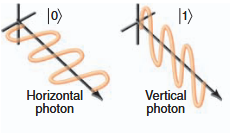
\includegraphics[width=0.5\linewidth]{Photonen_Polarisierung.png}
    \caption{Enter Caption}
    \label{fig:enter-label}
\end{figure}
\cite{obrien_optical_2007}

2. Time-Bin-Encoding 

Photons are chargeless particles, and do not interact very strongly with each other, or even with most matter. They can be guided along long distances with low loss in optical fibers, delayed efficiently using phase shifters, and combined easily using beamsplitters. Photons exhibit signature quantum phenomena, such as the interference produced in two-slit ex- periments. Furthermore, in principle, photons can be made to interact with each other, using nonlinear optical media which mediate interactions 

\textbf{In elektromagnetischem Resonator ist Energie nicht kontinuierlich sondern in units -> “Photonen” -> kleinste Einheiten von Licht / elektromagnetischer Strahlung. }

\textbf{Energiemenge eines Photons hängt von Frequenz der Schwingung ab ℏω (}das reduzierte Plancksche Wirkungsquantum, eine fundamentale Naturkonstant) 

-> in dem Resonator kann es null oder genau ein Photon geben (wie beim Qubit -> Superposition) 

 \cite{nielsen_quantum_2010}
 
\subsection{Spin-Qubits}

Spin-Qubits stellen eine der vielversprechendsten Realisierungen von Quantenbits dar, die auf dem fundamentalen quantenmechanischen Eigendrehimpuls, dem Spin, von Elektronen oder Atomkernen basieren. Im Wesentlichen repräsentieren die zwei möglichen Spinorientierungen eines Elektrons, häufig als \(\ket{\uparrow}\) (Spin-up) und \(\ket{\downarrow}\) (Spin-down) bezeichnet, die Basiszustände eines Qubits. Die Manipulation und Kontrolle dieser Zustände erfolgt durch gezielte Einwirkung von elektromagnetischen Feldern, etwa Mikrowellenpulsen oder lokal angelegten Magnetfeldern, die Spin-Resonanzphänomene ausnutzen.

Typischerweise werden Spin-Qubits in Halbleiterstrukturen realisiert, beispielsweise in Quantendots, die als künstliche Atome dienen und einzelne Elektronen in nanoskaligen Potentialmulden einschließen. Alternativ finden sich auch supraleitende Systeme oder Punktdefekte in Diamanten, wie NV-Zentren, als Plattformen für Spin-Qubits. Die Vorteile von Spin-Qubits liegen vor allem in ihren vergleichsweise langen Kohärenzzeiten – also der Zeitspanne, in der der Quanteninformationsträger seine Quanteneigenschaften ohne störende Einflüsse aus der Umgebung bewahrt – sowie in der Kompatibilität mit etablierten Halbleiterfertigungstechnologien, was die Integration in skalierbare Quantenprozessoren begünstigt.

Die Kopplung zwischen einzelnen Spin-Qubits, die zur Realisierung von Quantenlogikgattern erforderlich ist, erfolgt häufig über Austauschwechselwirkungen oder durch elektromagnetische Felder, welche kontrollierte Quantengatter ermöglichen. Trotz dieser Fortschritte stellt die hochpräzise Steuerung und Fehlerkorrektur eine zentrale Herausforderung dar, da Umwelteinflüsse und Rauschen leicht zu Dekohärenz und Informationsverlust führen können. Aktuelle Forschungsarbeiten konzentrieren sich daher auf die Verbesserung der Kohärenzzeiten, die Entwicklung von Fehlerkorrekturverfahren sowie die Skalierung der Systeme zu größeren Qubit-Anzahlen, um praktische Quantenrechner realisieren zu können.

\subsection{Neutralatom-Qubits}

Neutralatom-Qubits verwenden ungeladene Atome, die mittels optischer Fallen oder optischer Gitter auf sehr kleinen Skalen präzise positioniert und gehalten werden. Diese Atome bilden dabei die Informationsträger, wobei die Qubit-Zustände meist durch unterschiedliche hyperfeine Energiezustände innerhalb des Atoms definiert sind. Die hyperfeinen Zustände entstehen durch Wechselwirkungen zwischen dem Kernspin und dem Elektronenspin und bieten stabile und gut kontrollierbare Basiszustände \(\ket{0}\) und \(\ket{1}\) für das Qubit.

Die Manipulation der Qubits erfolgt in der Regel durch kohärente Laserpulse, welche Zustandsübergänge anregen oder kontrollierte Wechselwirkungen zwischen benachbarten Atomen induzieren. Besonders hervorzuheben sind sogenannte Rydberg-Zustände, bei denen ein Elektron eines Atoms in einen stark angeregten Zustand versetzt wird. Diese Rydberg-Zustände ermöglichen aufgrund ihrer stark erhöhten Wechselwirkungen eine effiziente Realisierung von Quantenlogikgattern zwischen neutralen Atomen, was sie für die Quanteninformationsverarbeitung sehr attraktiv macht.

Ein wesentlicher Vorteil von Neutralatom-Qubits liegt in der Skalierbarkeit der Systeme: Optische Gitter erlauben die Anordnung von Tausenden oder sogar Millionen von Atomen in regelmäßigen Gittern, was große Quantensysteme mit vielen Qubits ermöglicht. Darüber hinaus weisen diese Systeme vergleichsweise lange Kohärenzzeiten auf und profitieren von der hohen Homogenität und Reproduzierbarkeit der Atome. Allerdings stellen die exakte Positionierung der Atome, die Minimierung von Dekohärenzeffekten durch Umwelteinflüsse sowie die präzise Kontrolle der Wechselwirkungen technische Herausforderungen dar, an deren Lösung intensiv geforscht wird.

Insgesamt bilden Neutralatom-Qubits aufgrund ihrer Kombination aus Skalierbarkeit, Kontrollierbarkeit und Kohärenzzeit eine vielversprechende Plattform für die Entwicklung von Quantencomputern und Quanten-Simulatoren und ergänzen damit die auf Spin-Qubits basierenden Ansätze auf ideale Weise.





Zitat \cite{alhazmi_live_2024}

\cite{bergou_quantum_2021}

\printbibliography
